\documentclass[11pt,letterpaper]{article}
\usepackage[margin=0.85in]{geometry}
\usepackage[T1]{fontenc}
\usepackage{lmodern,microtype,amsmath,amssymb,graphicx,booktabs,longtable,array,caption,float,fancyhdr,xcolor}
\usepackage[hidelinks,hypertexnames=false]{hyperref}
\usepackage[section]{placeins}
\usepackage{enumitem}
\setlist{noitemsep,topsep=4pt}
\setlength{\parskip}{5pt}
\setlength{\parindent}{0pt}
\setlength{\emergencystretch}{2em}
\captionsetup{font=small,labelfont=bf}
\pagestyle{fancy}\fancyhf{}\fancyhead[L]{\small DBS optimization: ground-truth validation}\fancyhead[R]{\small Version 2}\fancyfoot[C]{\thepage}
\setlength{\headheight}{14pt}
\newcommand{\br}{\mathrm{BetaRatio}}
\newcommand{\Aeff}{A_{\mathrm{eff}}}
\newcommand{\fd}{Surrogate (Full-Domain)}
\makeatletter
\setlength{\@fptop}{0pt}
\makeatother
\begin{document}
\begin{titlepage}
\centering
\vspace*{1.1in}
{\LARGE\bfseries Benchmarking Quantum-Assisted Optimization for Parkinson's Deep Brain Stimulation:\par A Ground-Truth Validation Study\par}
\vspace{0.7in}
{\Large Version 2\par}
\vspace{0.15in}
{\large October 2026 Validated Revision\par}
{\large October 4, 2026\par}
\vfill
\begin{minipage}{0.88\textwidth}
\textbf{Version note.} This manuscript is a substantial validated revision of the March 2026 study, \emph{Quantum-assisted Optimization of Parkinson's Deep Brain Stimulation (DBS) Parameters}. It supersedes the original Stage 3 conclusions following methodological re-audit. The March manuscript remains preserved as Version 1. Stages 1 and 2 retain their historical results, with source and validation-scope qualifications stated explicitly. The corrected Stage 3 evidence is frozen at commit:\par
\smallskip
\small\nolinkurl{a94acf521bc596583b873283a509b43418b0fb76}\par
\normalsize\smallskip
This is a simulation-based research benchmark. No patient treatment, anatomical electrode reconstruction, or quantum-hardware experiment is reported.
\end{minipage}
\vspace{0.5in}
\end{titlepage}

\begin{abstract}
Parkinson's deep brain stimulation (DBS) programming combines interacting stimulation parameters with efficacy, energy, and safety considerations under limited opportunities to evaluate settings. We study this constrained search through a classical subthalamic nucleus--external globus pallidus (STN--GPe) simulator, normalized beta-band power, and brute-force ground truth. A three-stage benchmark compares classical optimizers and a surrogate-to-QUBO-to-simulated-QAOA proposal pipeline at evaluation budgets of 10, 20, 30, and 40. Historical Stage 1 results favor CMA-ES for smooth frequency--amplitude--pulse-width tuning; the reported QAOA gap narrows in the constrained Stage 2 extension. The validated Stage 3 study uses 16 binary contact variables, exactly six active contacts, and a fitted-efficacy screen admitting 6,881 masks. Across 30 seeds, corrected simulated $p=1$ QAOA remains competitive in objective-query efficiency but is not statistically separated from full-domain classical surrogate search at any budget (all four Holm-adjusted $p=1.000$). Exhaustive binary-QUBO/Ising checks agree to floating-point precision, and all 1,830 adaptive proposals originate from QAOA samples, with no fallback. However, direct-simulator validation exposes substantial local distortion in the quadratic efficacy approximation, and cardinality sensitivity does not support a physiological requirement for six contacts. Classical optimization remains strongest in the reported smooth-tuning benchmark. Greater constraint and combinatorial structure motivate further comparison, but do not establish superiority of the quantum-assisted method. Benchmark design, biological model fidelity, implementation verification, and strong classical comparison are necessary guardrails for evaluating quantum-assisted medical optimization.
\end{abstract}

\textbf{Keywords:} Parkinson's disease; deep brain stimulation; ground-truth benchmarking; surrogate optimization; QAOA; model validation.

\section{Introduction and related work}
DBS programming requires choosing stimulation frequency, amplitude, pulse width, and contact configuration while balancing therapeutic response, adverse effects, and energy use. These interacting decisions are patient dependent, and each assessment consumes programming time and patient effort. Clinical programming algorithms organize this search, while semi-automated optimization offers a complementary way to choose informative settings \cite{picillo,louie}. The relevant computational question is how to make useful decisions from limited evaluations, rather than how to optimize an unconstrained mathematical objective in isolation.

Beta-band activity provides one measurable link between stimulation and basal-ganglia dynamics. Wang et al. observed suppression of pallidal beta activity and pallidal--motor-cortex coherence during therapeutic stimulation \cite{wang}. This motivates beta power as a modeling proxy, but does not make it a complete measure of clinical benefit. A lower simulated beta ratio is not a demonstrated improvement in motor function, gait, speech, cognition, or quality of life.

Classical DBS optimization already has empirical support. Louie et al. studied Bayesian optimization of stimulation frequency using quantified rigidity in two participants, alongside a model of patient preferences \cite{louie}. Their restricted proof of concept supports algorithmic programming research; it does not validate the synthetic objectives used here. Fleming et al. developed time-adaptive Bayesian optimization for a computational neurostimulation model, illustrating why changing response landscapes matter for future adaptive systems \cite{fleming}.

Quantum-related biomedical work addresses distinct tasks. Vatsavai et al. investigated quantum-inspired multimodal Parkinson's screening \cite{vatsavai}; Ngo et al. developed QOMIC for motif identification in biological networks \cite{ngo}. Neither establishes efficacy for DBS parameter optimization. QAOA, introduced by Farhi et al., supplies a variational framework for proposing solutions to discrete optimization problems \cite{farhi}. Encoding a problem as a quadratic unconstrained binary optimization (QUBO) model makes such a comparison possible, but does not establish that the encoding favors quantum computation.

This study asks under what problem structures a quantum-assisted proposal layer is useful relative to strong classical alternatives. Weak baselines, inappropriate admissibility rules, or an inaccurate efficacy model can make an optimizer appear attractive for reasons unrelated to useful search behavior. We therefore treat domain validation, implementation verification, and strong-baseline comparison as parts of the scientific contribution. The study evolves from smooth tuning through clinically motivated constraints to a controlled combinatorial benchmark; it does not assume an inevitable transition to quantum superiority.

\section{Research questions and study scope}
The primary question is: \emph{Under limited objective-evaluation budgets, how does a simulated QAOA-assisted surrogate proposal method compare with strong classical optimizers for Parkinsonian DBS tuning as the problem becomes increasingly constrained, discrete, and combinatorial?}

Three secondary questions guide interpretation: (1) How does descriptive optimizer ranking change with problem structure? (2) Does QAOA remain competitive against a strong full-domain classical surrogate proposal mechanism? (3) How sensitive are Stage 3 conclusions to admissibility and efficacy-model fidelity?

The three stages form one research program, but are not a controlled ablation in which only problem structure changes. Objectives, encodings, and historical optimizer implementations differ. The Stage 3 correction and validation do not retroactively validate the Stage 1/2 quantum routines. Their original results are retained as descriptive context; formal comparative inference in this revision is centered on the corrected Stage 3 experiment. No research code was changed and no optimizer experiment was rerun for this manuscript.

\section{Methods}
\subsection{Classical STN--GPe model and efficacy measurement}
The unchanged simulator is a two-population delayed-feedback model with STN excitation of GPe and GPe inhibition of STN. For activities $s(t)$ and $g(t)$, its deterministic dynamics have the form
\begin{align}
\tau_s\dot{s}(t)&=-s(t)+\tanh\!\left[G_s\{I_c-w_{gs}g(t-d_{gs})+I_{\mathrm{DBS}}(t)\}\right],\\
\tau_g\dot{g}(t)&=-g(t)+\tanh\!\left[G_g\{w_{sg}s(t-d_{sg})+I_g\}\right].
\end{align}
DBS is a periodic rectangular pulse train in the STN input. The model uses forward Euler integration for 2 s with a 0.1 ms step, discards the first 0.2 s, and analyzes $s-g$. Initial activities are both 0.1, delays are discretized to simulation steps, and stochastic drive is zero. Fixed parameters appear in Appendix~\ref{app:params}. The no-stimulation peak is approximately 19.53 Hz, within the 13--30 Hz beta band.

Welch power spectral density estimation uses segments of at most 8,192 samples; beta power is integrated over 13--30 Hz. The efficacy ratio is
\begin{equation}
\br=\frac{P_{13\text{--}30\,\mathrm{Hz}}(\mathrm{DBS})}{P_{13\text{--}30\,\mathrm{Hz}}(\mathrm{baseline})}.
\end{equation}
Lower values indicate greater suppression in this simulator. Amplitude is in model units, not calibrated clinical milliamperes or volts. The model is a controlled oscillatory testbed, not a patient-specific biophysical reconstruction.

\subsection{Stages 1 and 2: preserved benchmark design}
Stage 1 spans 64 frequencies from 60 to 180 Hz, 64 amplitudes from 0 to 1.5 model units, and 16 pulse widths from 50 to 240 $\mu$s: 65,536 settings in total. Exhaustive simulation provides an oracle. The normalized energy proxy is $E=(A/1.5)^2(f/180)(PW/240\,\mu\mathrm{s})$. A Pareto front over beta ratio and energy supplies a knee energy $E_{\mathrm{knee}}$. The scalar objective is
\begin{equation}
J_{1,2}=\br+5\max(0,E-E_{\mathrm{knee}}).
\end{equation}
The knee minimizes Euclidean distance to the ideal origin in min--max-normalized beta-ratio/energy coordinates. Ground truth is the minimum of this specified scalar objective, not a uniquely established clinical tradeoff.

Stage 2 adds ring versus directional contact mode, producing 131,072 settings. Synthetic area factors are 1.0 and 0.25, impedance factors 1.0 and 2.0, and amplitude-focus factors 1.0 and 1.4, respectively. The normalized charge-density proxy is $(A/1.5)(PW/240\,\mu\mathrm{s})/\mathrm{area}$; settings above 0.60 are excluded from the feasible ground-truth calculation. Energy includes the impedance factor, and efficacy uses the focus-scaled amplitude. These are clinically motivated modeling assumptions, not validated safety limits or anatomical electric-field calculations. There are 77,504 feasible settings.

Both stages compare Random, Genetic Algorithm (GA), Bayesian Optimization (BO), CMA-ES, a classical quadratic-surrogate proposal method, and the historical QAOA-assisted pipeline. CMA-ES is a covariance-adaptation method for continuous search \cite{hansen}, rounded to the parameter grid in these stages. The Stage 1 classical surrogate scans its full grid; the Stage 2 version uses a 5,000-candidate pool. We therefore replace the ambiguous historical label ``Surrogate (Exact)'' with stage-specific names. Stages 1/2 use binary encodings of grid indices; Stage 3 bits directly represent selected synthetic contacts. Historical QAOA phase construction and sparsification differ from corrected Stage 3; the scope implications are discussed in Section~\ref{sec:limits}.

\subsection{Stage 3: fixed-cardinality, efficacy-screened contact selection}
Stage 3 isolates contact selection at 130 Hz and 240 $\mu$s. Sixteen binary variables $x_i\in\{0,1\}$ describe one hand-specified synthetic contact-metadata instance. Focus, risk, impedance, area, and pairwise-overlap values introduce heterogeneous linear and pair interactions. Indices are identifiers, not anatomical electrode positions. Even the circular index-distance rule used to construct overlaps is synthetic, not a physical lead geometry.

Effective amplitude is $\Aeff=0.25\sum_{i=0}^{15}F_i x_i$. A quadratic least-squares approximation, originally fit to 41 simulator amplitudes from 0 to 4, retains a QUBO-compatible efficacy term:
\begin{equation}
\widehat{\br}(A)=0.9437580303537102-0.11458817038088676A+0.022290112770454024A^2.
\label{eq:fit}
\end{equation}
This fixed efficacy approximation is distinct from the \emph{adaptive learned surrogate} fit to queried total objective values by the proposal methods. Confusing these two approximations would obscure both the model-validation and optimizer comparisons.

The primary admissible domain is
\begin{equation}
\mathcal D_6=\left\{x:\sum_i x_i=6,\quad\widehat{\br}(\Aeff)\leq0.8228585\right\}.
\end{equation}
The threshold is inherited from the Stage 2 knee efficacy. Exactly six contacts is a benchmark design choice that produces a nontrivial combinatorial domain under the fitted model. It does not establish clinical or physiological necessity. The full 65,536-mask space contains 8,008 exactly-six masks, of which 6,881 are fitted-admissible.

With $c_0$ the intercept in Equation~\ref{eq:fit}, the unchanged Stage 3 cost is
\begin{align}
J_3(x)={}&\widehat{\br}(\Aeff)-c_0+0.18\sum_i x_i
+0.20(0.25)^2\sum_i I_i x_i\nonumber\\
&+0.22\sum_i R_i x_i+0.30\sum_{i<j}O_{ij}x_ix_j
+0.40\sum_i q_i x_i,\\
q_i={}&\left[\max\!\left(0,\frac{0.25/1.5}{\mathrm{area}_i}-0.55\right)\right]^2.
\end{align}
Here $I_i,R_i,O_{ij}$ are synthetic impedance, risk, and overlap factors. Metadata and construction rules are given in Appendix~\ref{app:params}. The charge-density soft term is zero for this instance; the count term is constant at fixed $k=6$. Both remain in the frozen definition. The omitted efficacy intercept cancels from regret. These terms are benchmark proxies, not calibrated estimates of battery life or patient harm.

\subsection{Ground truth, budgets, and classical comparators}
Exhaustive offline evaluation defines $J^*=\min_{x\in\mathcal D_6}J_3(x)$. Performance after $B$ queries is simple regret, $r_B=\min_{t\leq B}J_3(x_t)-J^*$. All seven Stage 3 methods receive $B\in\{10,20,30,40\}$ unique selected objective queries, with 30 seeds (0--29) per method and budget. In this experiment, a ``true-objective query'' is a query to the fixed fitted Stage 3 cost cached in an offline oracle. It is not a fresh neural simulation or a patient trial. The query budget models scarcity of informative evaluations; its numerical values are not empirically calibrated clinical programming limits.

Offline enumeration, efficacy-fit preparation, admissibility screening, surrogate predictions, optimizer computation, and model-validation simulations are outside $B$. This separation makes objective-query efficiency measurable without claiming equal computation. All methods share the same admissibility screen, and all 21,000 selected observations across 840 runs are admissible and meet their exact budgets.

Random draws unseen admissible masks. GA uses a budget-dependent population of 8--16 before the $B-2$ cap, elite selection, uniform crossover, and independent bit mutation with probability $0.3/16$, rejecting inadmissible offspring. BO fits a normalized Gaussian process with a Mat\'ern-$5/2$ kernel and selects expected improvement ($\xi=0.01$) over 4,000 admissible continuous proposals decoded by a 0.5 threshold. CMA-ES uses 16 continuous coordinates, initial mean 0.5, initial scale 0.35, and population 18, with threshold decoding and admissibility rejection. These implementations remain fixed; the comparison is not an exhaustive search over classical algorithm designs.

The three surrogate methods fit $\widehat J(x)=c+\sum_i a_i x_i+\sum_{i<j}b_{ij}x_ix_j$ using 137 features and ridge coefficient 0.001, including intercept regularization. They share exactly the same initial masks and costs for each seed and budget: nine at $B=10$, ten otherwise. Subsequent histories evolve independently.

\emph{Surrogate (Pool)} makes 5,000 random admissible candidate draws per adaptive step, skips evaluated masks, and selects the minimum surrogate prediction. Draws can repeat; this is not 5,000 guaranteed distinct candidates. \emph{\fd} scores the learned surrogate over every currently admissible, unevaluated mask and selects the minimum, breaking exact ties by lowest integer mask. It then spends only \emph{one} true-objective query on that proposal. Full-domain surrogate scoring is cheap candidate evaluation, not exhaustive DBS testing, and exact minimization of a learned prediction is not exact minimization of the underlying objective.

\subsection{Corrected QUBO-to-Ising transformation and circuit verification}
For the complete binary quadratic expression $f(x)=c+\sum_i a_ix_i+\sum_{i<j}b_{ij}x_ix_j$, substitute
\begin{equation}
x_i=\frac{1-Z_i}{2},\qquad x_ix_j=\frac{1-Z_i-Z_j+Z_iZ_j}{4}.
\end{equation}
The resulting Ising form is $H=C+\sum_i h_iZ_i+\sum_{i<j}J_{ij}Z_iZ_j$, where
\begin{equation}
J_{ij}=b_{ij}/4,\quad h_i=-a_i/2-\tfrac14\sum_{j\ne i}b_{ij},\quad
C=c+\tfrac12\sum_i a_i+\tfrac14\sum_{i<j}b_{ij}.
\end{equation}
The incident-pair sum uses the appropriate upper-triangular coefficient for each pair. All terms present in the fitted binary surrogate are transformed before circuit construction. Cost gates use $R_Z(2\gamma h_i)$ and $R_{ZZ}(2\gamma J_{ij})$; $C$ contributes only a global phase.

\textbf{Constraint handling is separate.} The frozen phase QUBO contains no quadratic cardinality penalty or fitted-efficacy constraint penalty. Hard admissibility is enforced by classical filtering. During angle optimization, inadmissible or already-seen samples receive a rejection score of 1,000 in the sampled classical expectation, not in the phase Hamiltonian. It would therefore be incorrect to claim that hard constraints were transformed into the circuit. The recorded bound $|c|+\sum|a_i|+\sum|b_{ij}|$ never exceeds 10.502754, so the rejection score exceeds every possible admissible surrogate prediction. The X mixer does not preserve cardinality.

Three exhaustive energy checks each cover all 65,536 binary states: the true objective, an initial learned surrogate, and an asymmetric test fixture. The maximum discrepancy across checks is $2.84217\times10^{-14}$ and the mean absolute discrepancy across all three full-space checks is $1.58893\times10^{-15}$. The actual cost-plus-mixer circuit also agrees with direct statevector evolution to a maximum discrepancy of $6.05913\times10^{-17}$. Bit $i$ corresponds to contact/qubit $i$; displayed strings are most-significant-bit first. These tests validate implementation correctness to floating-point precision; they do not establish optimizer superiority.

\subsection{Simulated hybrid QAOA-assisted proposals and attribution}
The adaptive pipeline comprises classical surrogate fitting, binary QUBO construction, the corrected Ising mapping, classical angle optimization, simulated $p=1$ QAOA sampling, admissibility filtering, and evaluation of the selected proposal. Sixteen qubits start in a Hadamard superposition, receive all 120 pair interactions and independent $R_X(2\beta)$ mixers, and are measured. The circuit optimizes a learned quadratic cost; the STN--GPe dynamics remain entirely classical.

Angles start uniformly in $[0,\pi]$ from the seeded random generator. COBYLA uses at most 30 sampled objective evaluations with 256 shots each. A final 1,024-shot batch supplies candidate masks; the unseen admissible sample with minimum predicted cost is queried. A preserved 5,000-draw classical fallback would be used if none were available. Proposal-source instrumentation records which path actually supplies each query.

All 1,830 adaptive proposals came from QAOA samples (1,830/1,830); the fallback rate is 0\%. This rules out hidden fallback as the source of the reported performance. It does not isolate a causal advantage of quantum evolution: ridge fitting, COBYLA, rejection, filtering, and minimum-prediction selection remain integral classical components. A same-history diagnostic computes the full-domain surrogate minimum using each QAOA training history without querying that diagnostic mask; it is distinct from the independent adaptive comparator.

Across 120 QAOA runs, 3,000 budgeted queries comprise 1,170 initialization queries and 1,830 adaptive queries. Internal sampling uses 52,999 angle-search circuits plus 1,830 final circuits: 54,829 circuits and 15,441,664 shots. There are also 1,830 diagnostic statevector evaluations and same-history prediction scans, not used for proposal selection. Equal objective-query budgets therefore do not imply equal computational cost. No quantum hardware or runtime speedup is demonstrated.

\subsection{Statistics and model-sensitivity analysis}
Stage 3 summaries report mean, population SD ($ddof=0$), median, IQR, range, and seed-level 95\% percentile-bootstrap mean intervals with 10,000 resamples. The principal comparison pairs QAOA and \fd\ by seed and matched initialization. The paired difference is QAOA regret minus comparator regret, so negative values favor QAOA. Paired bootstrap intervals resample complete pairs. Two-sided sign randomization is exact when at most 16 differences are nonzero; otherwise it uses 100,000 randomizations with plus-one correction. Ties use absolute tolerance $10^{-12}$. Holm correction covers the four principal budget comparisons. The secondary Pool comparison uses a separate four-budget family. Nonsignificance is interpreted as non-separation, not equivalence.

The fixed efficacy approximation is checked against the unchanged direct simulator on 401 amplitudes from 0 to 4 and 129 amplitudes over the full $k=6$ reachable interval, 1.40--1.72. It is not refit to the validation data. All masks additionally receive cached direct-model efficacy at their exact effective amplitudes. Sensitivity enumeration at $k=4,5,6,7$ changes only the cardinality used for model comparison; it does not replace the primary optimizer domain. No optimizer sweep is performed for those alternative cardinalities.

\section{Results}
\subsection{Stage 1: classical dominance in the reported smooth-tuning benchmark}
The Stage 1 Pareto front contains 109 nondominated settings (Figure~\ref{fig:s1}). Its knee and scalar optimum occur at approximately $f=176.19$ Hz, $A=0.667$, and $PW=227.33\,\mu$s, with $J^*=0.7844227120082152$. Table~\ref{tab:s1} preserves the March manuscript's complete four-budget results. CMA-ES has the lowest reported mean regret at every budget, falling from $0.0905\pm0.0276$ to $0.0478\pm0.0209$. Historical QAOA falls from $0.1039\pm0.0342$ to $0.0799\pm0.0387$. GA is next strongest at higher budgets. This supports classical dominance in the reported smooth low-dimensional setting, subject to the historical-protocol scope qualification.
\begin{table}[htbp]\centering
\caption{Stage 1 reported mean regret $\pm$ SD. Values preserved from Version 1 Table 1, p.~13; the corresponding sweep seed count is unverified.}\label{tab:s1}
\scriptsize
\setlength{\tabcolsep}{4pt}
\begin{tabular}{lrrrr}\toprule
Method & $B=10$ & $B=20$ & $B=30$ & $B=40$ \\ \midrule
Random & $0.1018\pm0.0346$ & $0.0893\pm0.0286$ & $0.0679\pm0.0254$ & $0.0673\pm0.0227$ \\
GA & $0.1067\pm0.0357$ & $0.0847\pm0.0334$ & $0.0662\pm0.0284$ & $0.0595\pm0.0273$ \\
BO & $0.1081\pm0.0313$ & $0.0904\pm0.0321$ & $0.0835\pm0.0341$ & $0.0693\pm0.0365$ \\
CMA-ES & $0.0905\pm0.0276$ & $0.0742\pm0.0263$ & $0.0586\pm0.0252$ & $0.0478\pm0.0209$ \\
Surrogate (Full-Domain) & $0.1039\pm0.0342$ & $0.0906\pm0.0420$ & $0.0789\pm0.0417$ & $0.0710\pm0.0434$ \\
QAOA (historical) & $0.1039\pm0.0342$ & $0.0936\pm0.0404$ & $0.0781\pm0.0406$ & $0.0799\pm0.0387$ \\
\bottomrule\end{tabular}
\end{table}

\begin{figure}[htbp]\centering
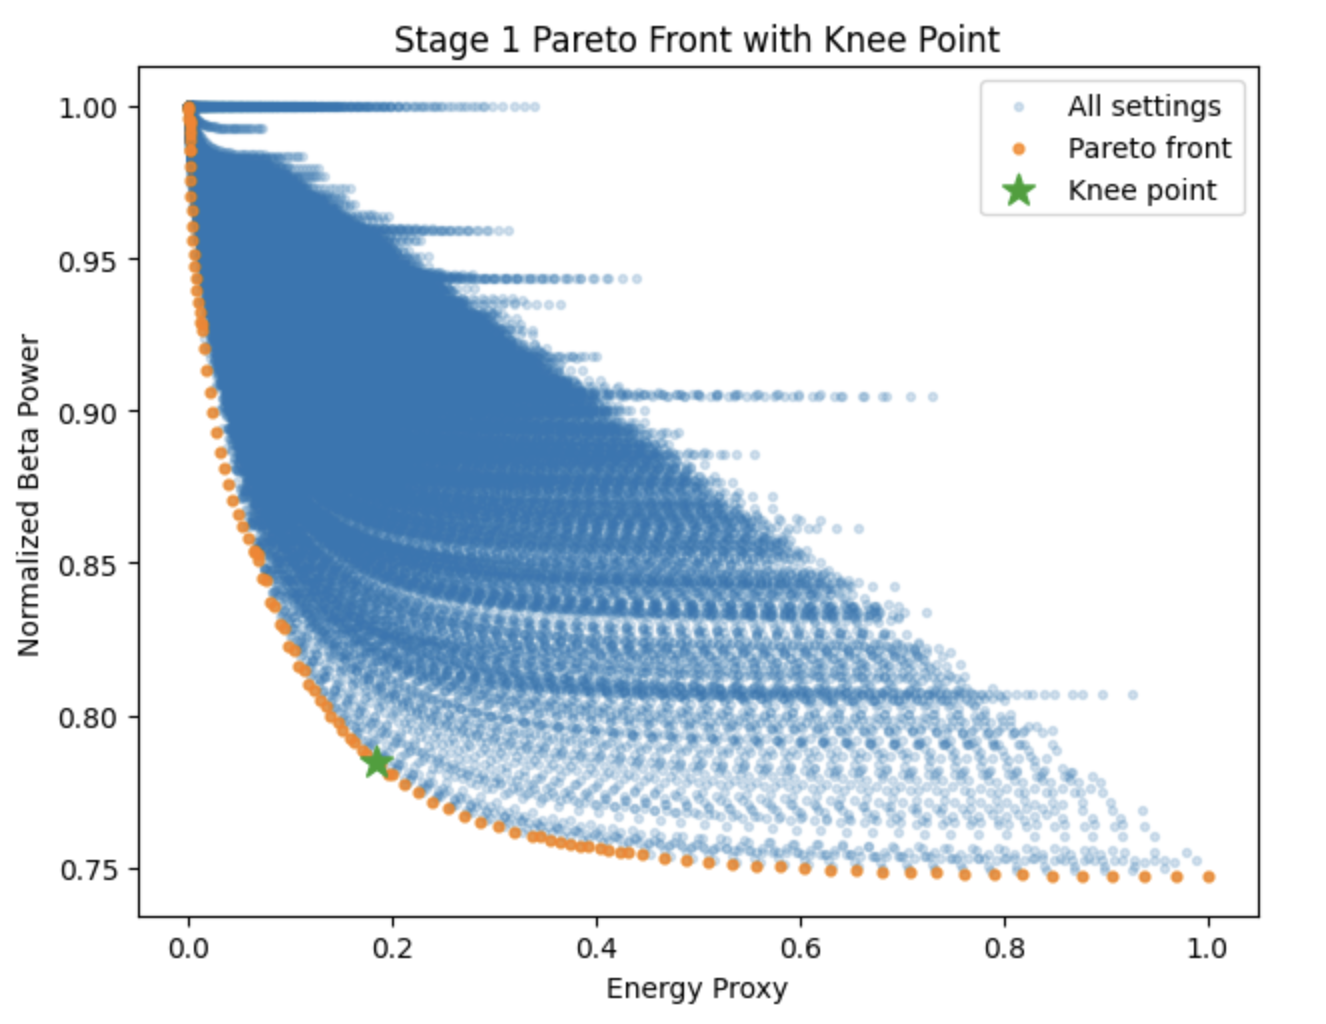
\includegraphics[width=0.67\textwidth]{figures/stage1_pareto_v1.png}
\caption{Stage 1 efficacy--energy Pareto front, extracted from the preserved March manuscript (original Figure 3, p.~12). Blue points show normalized beta-power/energy pairs from the 65,536-setting grid, orange points show the nondominated Pareto front, and the marked knee defines the scalar objective's energy reference. This is a simulator tradeoff, not a clinical therapeutic window.}\label{fig:s1}
\end{figure}

\subsection{Stage 2: narrowing descriptive performance gap}
The Stage 2 optimum is a ring-mode setting near $f=159.05$ Hz, $A=0.5$, and $PW=240\,\mu$s, with $J^*=0.8228584997287205$. CMA-ES again has the lowest mean regret at all budgets: 0.0839, 0.0749, 0.0658, and 0.0602. Historical QAOA means are 0.0974, 0.0860, 0.0751, and 0.0659 (Table~\ref{tab:s2}; Figure~\ref{fig:s2}). At $B=40$, the descriptive gap to CMA-ES is 0.0057, compared with 0.0321 in Stage 1. This comparison suggests greater competitiveness in the constrained extension, but is not a formal cross-stage treatment effect and does not guarantee superiority as complexity increases.

The frozen Stage 2 notebook's 30-seed sweep agrees with Version 1's results prose. Its table image contains conflicting values, including CMA-ES and QAOA entries. We retain the notebook/prose-consistent sweep throughout Version 2; the provenance audit records the discrepancies. Stage 1's four-budget table is preserved from Version 1 because the frozen notebook stores only separate single-budget summaries, not the corresponding sweep records. Its sweep-specific seed count cannot be verified from the supplied sources; no paired inference is inferred from that table.
\begin{table}[htbp]\centering
\caption{Stage 2 reported mean regret $\pm$ SD. Frozen notebook cell 16, 30 seeds; these values agree with Version 1 prose and replace its inconsistent table image.}\label{tab:s2}
\scriptsize
\setlength{\tabcolsep}{4pt}
\begin{tabular}{lrrrr}\toprule
Method & $B=10$ & $B=20$ & $B=30$ & $B=40$ \\ \midrule
Random & $0.1033\pm0.0242$ & $0.0841\pm0.0263$ & $0.0736\pm0.0205$ & $0.0696\pm0.0224$ \\
GA & $0.0998\pm0.0339$ & $0.0827\pm0.0248$ & $0.0775\pm0.0240$ & $0.0721\pm0.0245$ \\
BO & $0.1194\pm0.0280$ & $0.0995\pm0.0306$ & $0.0827\pm0.0310$ & $0.0683\pm0.0306$ \\
CMA-ES & $0.0839\pm0.0240$ & $0.0749\pm0.0246$ & $0.0658\pm0.0181$ & $0.0602\pm0.0202$ \\
Surrogate (Pool) & $0.0979\pm0.0270$ & $0.0948\pm0.0207$ & $0.0912\pm0.0220$ & $0.0883\pm0.0223$ \\
QAOA (historical) & $0.0974\pm0.0237$ & $0.0860\pm0.0205$ & $0.0751\pm0.0188$ & $0.0659\pm0.0244$ \\
\bottomrule\end{tabular}
\end{table}

\begin{figure}[htbp]\centering
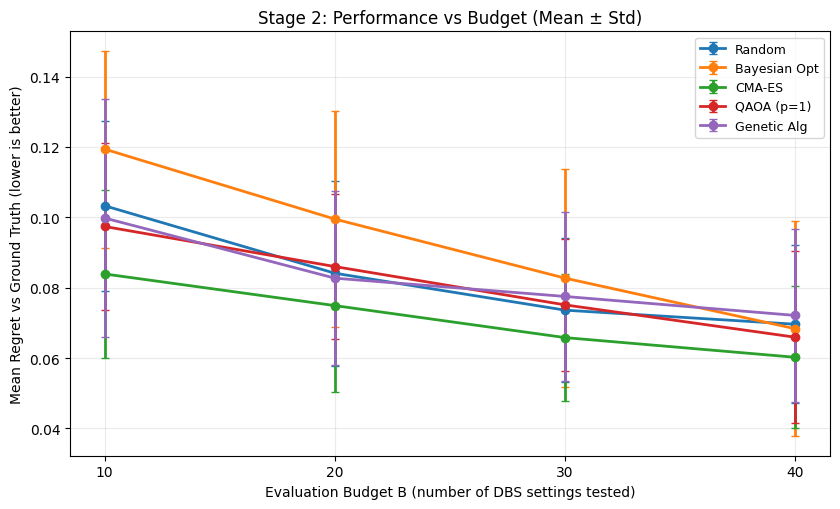
\includegraphics[width=0.78\textwidth]{figures/stage2_performance_saved.png}
\caption{Stage 2 historical optimizer performance, extracted from the stored output of \texttt{stage2.ipynb}, cell 17 (zero-based). Means and $\pm1$ population SD describe 30 runs at each budget for five displayed methods; Table~\ref{tab:s2} includes the classical surrogate pool. The horizontal axis counts benchmark settings, not observed patient trials. No optimizer was rerun for this figure.}\label{fig:s2}
\end{figure}

\subsection{Stage 3 ground truth and complete optimizer comparison}
The unique fitted-admissible optimum is mask 38180, binary \texttt{1001010100100100}, with zero-based active indices $[2,5,8,10,12,15]$. Its effective amplitude is 1.57; fitted beta ratio is 0.8187975018236102; total objective is 1.5690394714699. The direct-simulator beta ratio at this mask is 0.8149348670459028, used for validation only. This is an exact optimum of the specified fitted benchmark, not an optimal patient treatment. Objective components appear in Appendix~\ref{app:params}.

Table~\ref{tab:s3} includes all seven methods and all four budgets. Appendix~\ref{app:descriptive} supplies the complete validated descriptive table, including medians, IQRs, ranges, ranks, and bootstrap intervals. Random has the lowest descriptive mean at $B=10$; \fd\ at $B=20$; and Pool at $B=30$ and 40. QAOA ranks third, second, third, and second, respectively. Pool and Full-Domain tie at $B=10$, where only one adaptive query follows the nine shared initial observations.

At $B=40$, mean regret is 0.052564 for Pool, 0.058041 for QAOA, and 0.059358 for Full-Domain. Full-domain minimization of a learned surrogate need not yield the best realized objective trajectory: restricted candidate sampling can alter exploration. Here, competitive denotes the observed range of regret, not a formal equivalence or noninferiority margin. These descriptive ranks do not establish population-level superiority. Figure~\ref{fig:s3} shows the uncertainty in the mean estimates.
\begin{table}[htbp]\centering
\caption{Validated Stage 3 mean regret $\pm$ population SD, 30 seeds per cell. Pool and Full-Domain denote classical surrogate proposal methods; QAOA is the simulated hybrid $p=1$ method. All selected queries are admissible.}\label{tab:s3}
\scriptsize
\setlength{\tabcolsep}{4pt}
\begin{tabular}{lrrrr}\toprule
Method & $B=10$ & $B=20$ & $B=30$ & $B=40$ \\ \midrule
Random & $0.174012\pm0.063906$ & $0.144140\pm0.060162$ & $0.127619\pm0.048665$ & $0.113079\pm0.045784$ \\
GA & $0.205983\pm0.102295$ & $0.125186\pm0.060365$ & $0.099263\pm0.052292$ & $0.075283\pm0.038768$ \\
BO & $0.177022\pm0.080698$ & $0.128352\pm0.061696$ & $0.103829\pm0.043677$ & $0.082164\pm0.050326$ \\
CMA-ES & $0.184742\pm0.085346$ & $0.143246\pm0.069175$ & $0.109434\pm0.058656$ & $0.098881\pm0.048787$ \\
Pool & $0.179932\pm0.067134$ & $0.123577\pm0.061877$ & $0.066622\pm0.039385$ & $0.052564\pm0.038273$ \\
Full-Domain & $0.179932\pm0.067134$ & $0.111238\pm0.066653$ & $0.076354\pm0.039815$ & $0.059358\pm0.034858$ \\
QAOA (p=1) & $0.177592\pm0.069727$ & $0.122321\pm0.038240$ & $0.080358\pm0.047602$ & $0.058041\pm0.040225$ \\
\bottomrule\end{tabular}
\end{table}

\begin{figure}[htbp]\centering
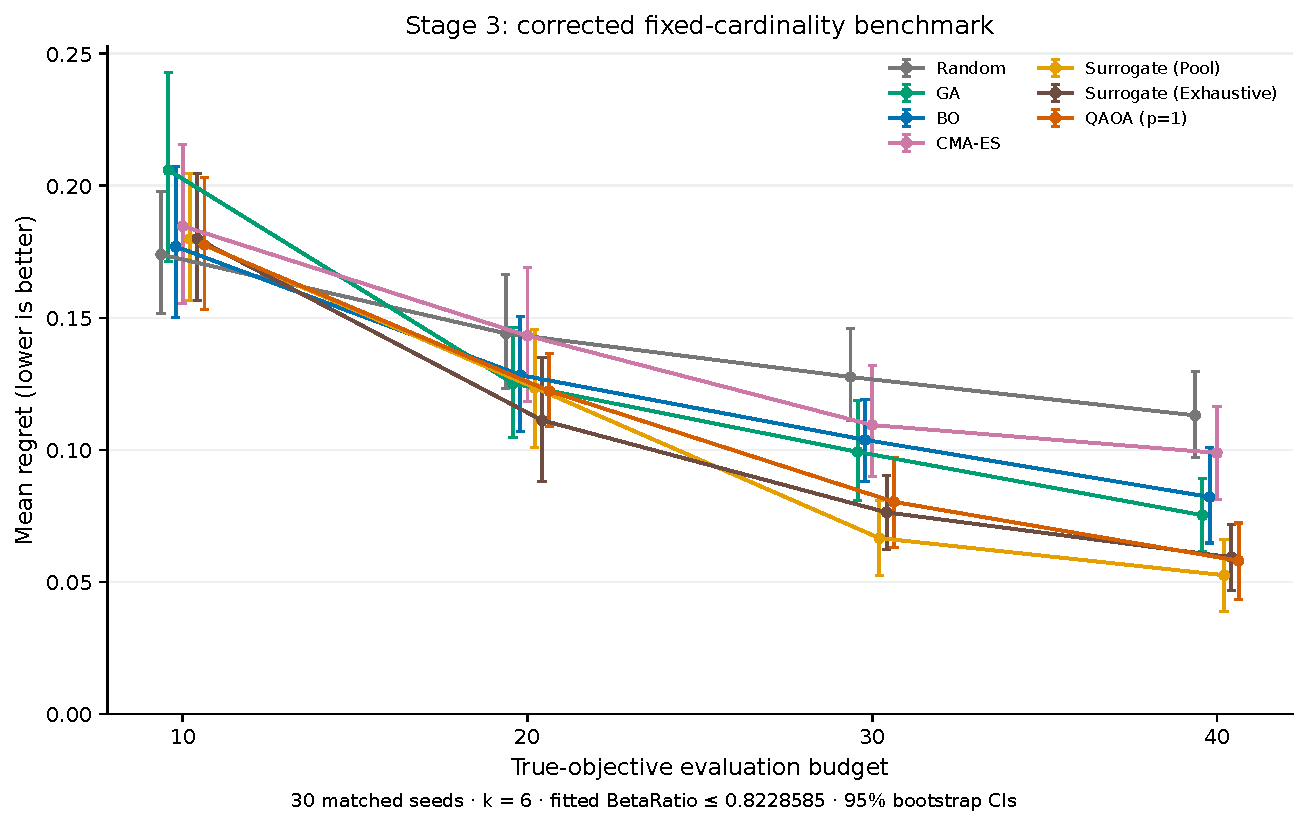
\includegraphics[width=0.92\textwidth]{figures/stage3_regret_vs_budget.pdf}
\caption{Validated Stage 3 mean simple regret versus budget, over 30 seeds per method/budget on one synthetic instance. Error bars are seed-level 95\% percentile-bootstrap confidence intervals (10,000 resamples), not SD. Small horizontal offsets separate intervals without changing budgets. ``Surrogate (Exhaustive)'' in the unchanged source artwork means \fd. Ground truth is the fitted-admissible minimum 1.5690394714699.}\label{fig:s3}
\end{figure}

\subsection{Principal paired comparison and QAOA attribution}
Table~\ref{tab:paired} gives all principal paired effects. QAOA has slightly lower mean regret than Full-Domain at $B=10$ and 40 and higher regret at $B=20$ and 30. Every paired interval includes zero; at $B=10$, the upper endpoint is zero and 28 of 30 pairs tie. All four Holm-adjusted $p$ values are 1.000. The methods are \emph{not statistically separated in this experiment}. This is not evidence of statistical equivalence, and no tested budget supports QAOA superiority over the principal comparator. The separate Pool comparison likewise gives no supported separation (Appendix~\ref{app:paired}).
\begin{table}[htbp]\centering
\caption{Paired QAOA minus Full-Domain (principal family). Negative favors QAOA. W/T/L counts QAOA wins/ties/losses across 30 seed pairs. All intervals include zero.}\label{tab:paired}
\scriptsize
\setlength{\tabcolsep}{4pt}
\begin{tabular}{lrrrrrr}\toprule
$B$ & Mean diff. & Median diff. & Paired 95\% CI & W/T/L & Raw $p$ & Holm $p$ \\ \midrule
10 & -0.002339 & 0.000000 & [-0.006991, 0.000000] & 2/28/0 & 0.500000 & 1.000 \\
20 & +0.011083 & +0.009333 & [-0.013820, +0.034628] & 9/6/15 & 0.382816 & 1.000 \\
30 & +0.004004 & +0.004567 & [-0.013226, +0.021094] & 14/1/15 & 0.651873 & 1.000 \\
40 & -0.001316 & -0.002231 & [-0.016504, +0.013464] & 15/2/13 & 0.867281 & 1.000 \\
\bottomrule\end{tabular}
\end{table}


Zero fallback accompanies a mean final-batch admissible-shot fraction of 18.934746\%; mean exact statevector admissible mass is 17.740169\%. Every selected query is admissible because filtering precedes evaluation. Raw sampled feasibility is therefore different from selected-query feasibility. QAOA selects the exact same-history full-domain surrogate minimizer in 70 of 1,830 steps (3.825\%); its mean selected-minus-minimum predicted-cost gap is 0.0877704473. These are surrogate diagnostics, not counterfactual true-objective results. Appendix figures show paired differences and the feasibility/fallback instrumentation.

\subsection{Dedicated efficacy-model validation}
The global quadratic fit has $R^2=0.761188$, but global fit quality does not ensure reliable local decisions. Over the $k=6$ reachable interval, $R^2=-986.838188$, RMSE is 0.005985589, and maximum absolute error is 0.011614132 (Table~\ref{tab:model}; Figure~\ref{fig:beta}). The strongly negative local $R^2$ is not a typographical error. The direct curve is nearly flat (approximately 0.814743--0.815409); the quadratic fails to track its small variation and performs worse by squared error than a constant predictor using the local direct mean. A small-looking absolute error can therefore materially distort admissibility.

The fitted downward threshold crossing is $A=1.482746$; the direct crossing is $A=0.923268$, a difference of 0.559478 amplitude units. The quadratic also crosses upward at approximately 3.658017, while the validated direct grid shows no corresponding upward crossing through $A=4$. That upturn is a fit artifact within the checked range. Direct-model validation reveals approximation error relative to a simplified simulator; it is not clinical validation of either the fitted curve or the inherited threshold.
\begin{table}[htbp]\centering
\caption{Fixed quadratic efficacy approximation versus direct simulation. Local $R^2$ reflects the nearly flat direct response; it is not a clinical validation metric.}\label{tab:model}
\small
\setlength{\tabcolsep}{4pt}
\begin{tabular}{lrrrrr}\toprule
Interval & $n$ & $R^2$ & RMSE & MAE & Maximum error \\ \midrule
Global $A=0$--4 & 401 & 0.761188 & 0.021294003 & 0.017489552 & 0.056353984 \\
Local $A=1.40$--1.72 & 129 & -986.838188 & 0.005985589 & 0.004834978 & 0.011614132 \\
\bottomrule\end{tabular}
\end{table}

\begin{figure}[htbp]\centering
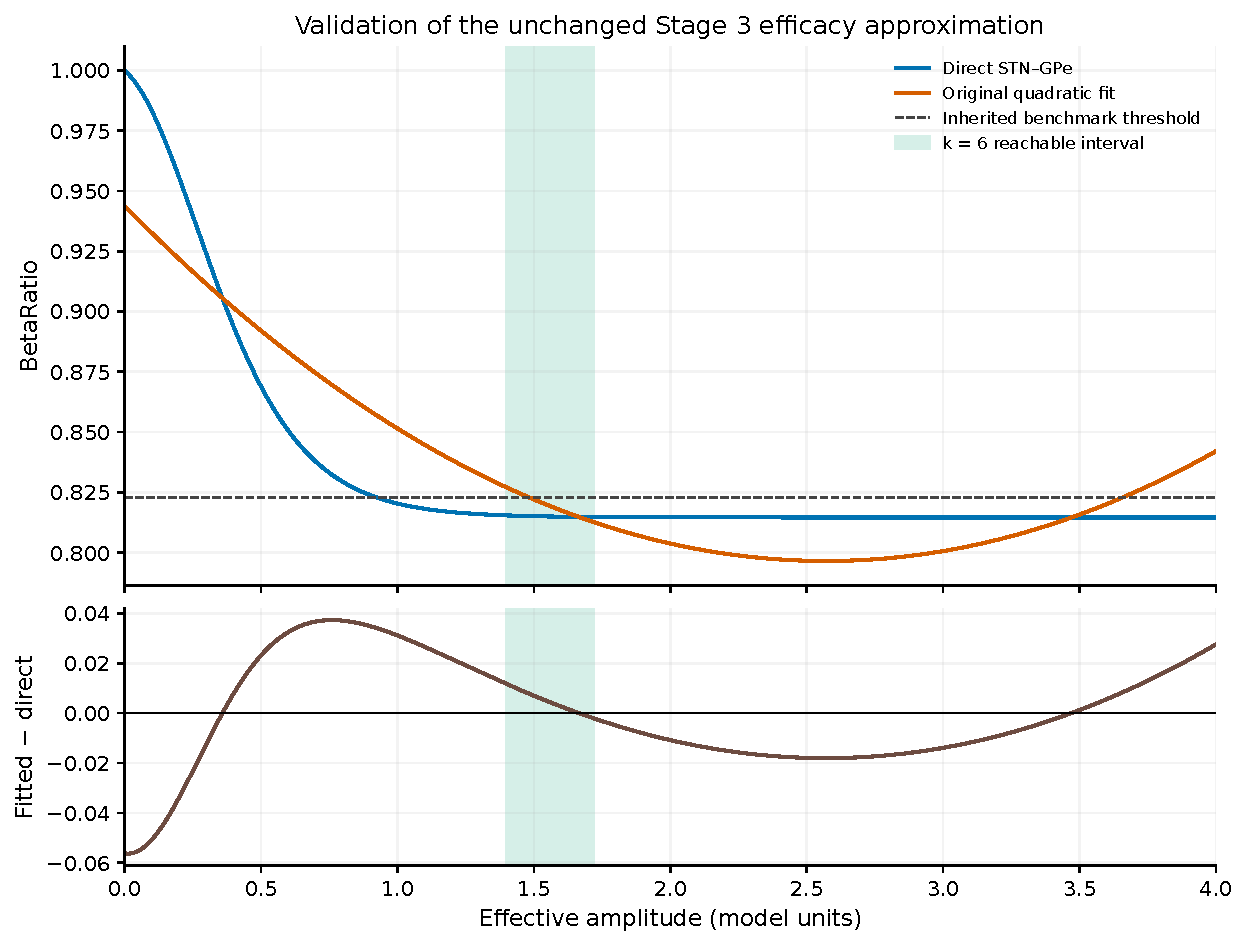
\includegraphics[width=0.93\textwidth]{figures/stage3_beta_fit_validation.pdf}
\caption{Unchanged quadratic efficacy fit versus the unchanged direct STN--GPe simulator on 401 amplitudes from 0 to 4. Shading marks the entire $k=6$ reachable interval, 1.40--1.72. Residuals are fitted minus direct beta ratio; local metrics use a separate 129-point grid. The inherited threshold 0.8228585 is a benchmark efficacy criterion, not a clinical treatment threshold.}\label{fig:beta}
\end{figure}

\subsection{Cardinality sensitivity}
At $k=4$, the fit accepts none of 1,820 masks whereas direct simulation accepts 1,817. At $k=5$, the fit accepts none of 4,368, while direct simulation accepts all. At $k=6$, the fit accepts 6,881 of 8,008 and direct simulation accepts all 8,008. At $k=7$, both accept all 11,440 (Table~\ref{tab:cardinality}). Thus 1,127 six-contact masks are rejected by the fit despite passing the direct criterion. These results do not support interpreting six contacts as physiologically or clinically necessary. We retain $k=6$ as a fixed-cardinality benchmark producing a nontrivial fitted-admissible domain. The sensitivity study is a domain/model check, not a new optimizer experiment.
\begin{table}[htbp]\centering
\caption{Sensitivity of inherited-threshold admissibility to cardinality and efficacy model. Counts enumerate every mask at each $k$.}\label{tab:cardinality}
\small
\setlength{\tabcolsep}{4pt}
\begin{tabular}{lrrrr}\toprule
$k$ & Masks & $A_{\mathrm{eff}}$ range & Fitted-pass & Direct-pass \\ \midrule
4 & 1,820 & 0.9200--1.2000 & 0 & 1,817 \\
5 & 4,368 & 1.1600--1.4625 & 0 & 4,368 \\
6 & 8,008 & 1.4000--1.7200 & 6,881 & 8,008 \\
7 & 11,440 & 1.6425--1.9750 & 11,440 & 11,440 \\
\bottomrule\end{tabular}
\end{table}


\section{Discussion}
\subsection{What changes as problem structure changes?}
The descriptive progression is classical dominance in smooth tuning, a narrowing historical gap with added constraints, and competitive corrected quantum-assisted performance in a discrete interaction-rich benchmark. CMA-ES is well matched to the reported low-dimensional smooth setting, while the Stage 3 surrogate methods use a representation aligned with the quadratic binary objective. This is a useful organizing observation, but not proof that increasing combinatorial structure causes a quantum benefit. The stage-specific objectives and implementations change together, and only Stage 3 receives the present corrected paired comparison.

The validated Stage 3 result is scientifically substantive even though it is non-separating. It shows that a correctly implemented simulated $p=1$ QAOA proposal method can remain competitive under a small query budget without relying on fallback, while a strong full-domain surrogate comparator removes the basis for a superiority claim. The original apparent 75--80\% Stage 3 regret advantage does not survive the corrected domain, implementation, and stronger comparison. The combined validation does not identify the separate causal contribution of each correction; it establishes what the final controlled evidence supports.

\subsection{Three distinct meanings of performance}
\textbf{Objective-query efficiency.} The relevant outcome is the regret remaining after a limited number of selected benchmark evaluations. On this measure, QAOA is competitive with the two classical surrogate strategies. Small descriptive differences change sign with budget, and paired uncertainty prevents claiming superiority over Full-Domain. The $B=10$ comparison is especially dominated by shared initialization.

\textbf{Computational cost.} The QAOA-assisted method requires classical fitting, angle optimization, filtering, and millions of simulated shots. Its 54,829 sampling circuits are additional work beyond the 3,000 counted queries. Classical full-domain prediction over 6,881 candidates is inexpensive at this scale. No matched-runtime benchmark or hardware-speedup experiment was performed, so equal query counts must not be interpreted as equal time, energy, or implementation complexity.

\textbf{Biological and clinical fidelity.} The oracle is exact for a fitted synthetic objective. It is not exact for the direct simulator's response and still less for clinical outcomes. The local efficacy mismatch changes which contact sets appear admissible. Consequently, excellent optimization of this oracle cannot establish better stimulation for a patient. This separation between optimization quality and objective validity is central to interpreting the experiment.

\subsection{Practical consequence: a decision framework}
At the present scale, the evidence does not justify choosing quantum optimization merely because contact selection admits a QUBO encoding. Strong classical optimization and full-domain surrogate scoring remain practical default comparators; this experiment supplies no statistically supported reason to prefer QAOA. This is a research-method selection conclusion, not a treatment recommendation.

Before introducing a quantum proposal layer into a safety-sensitive medical search, researchers should establish that the feasible domain is meaningful, the objective reflects the response being targeted, the binary-to-circuit implementation is correct, classical comparators are sufficiently strong, evaluation budgets are accounted for fairly, and apparent performance is attributed to the actual proposal path. The present experiment supplies concrete checks for each of these questions, including a case where model fidelity fails despite numerically correct optimization machinery.

Patient assessments and programming evaluations are scarce in real DBS, so sample efficiency is an appropriate motivation. It is insufficient if the learned objective misrepresents therapeutic response. An optimizer cannot compensate for a poorly validated objective. In this study, verifying the efficacy screen changes the interpretation more fundamentally than moving a method up or down a descriptive regret ranking.

\subsection{Why quantum-assisted proposals may still merit future study}
This result does not rule out future usefulness. The current admissible domain has only 6,881 masks, allowing cheap exhaustive surrogate prediction. Combinations of more contacts, multi-level current allocation, polarity, current steering, frequency, pulse width, impedance interactions, anatomical targeting, side-effect constraints, patient-specific models, temporal stimulation policies, and closed-loop adaptation could produce much larger domains. Full-domain candidate scoring may then become impractical.

That is a scaling hypothesis, not a demonstrated transition. Larger domains also permit stronger classical approximations, structured search, and better surrogate models; they do not automatically favor QAOA. Renewed comparisons should test whether a quantum-assisted proposal layer improves outcomes relative to those alternatives after all supporting computation and model assumptions are counted.

\section{Limitations}\label{sec:limits}
This is a simulation-based, preclinical benchmark using a simplified STN--GPe model. Beta power is a biomarker/proxy rather than a complete clinical outcome. Fixed simulation duration, time discretization, deterministic parameters, and synthetic risk/energy proxies constrain biological interpretation. No patient data, reconstructed electrode anatomy, or clinically validated efficacy/safety thresholds are supplied.

Stage 3 uses one synthetic metadata instance and an imperfect quadratic efficacy approximation. The fixed $k=6$ domain is artificial, and its threshold rejects direct-simulator-acceptable masks. Thirty seeds quantify optimizer randomness on one landscape; they do not measure variability across patients or instances. The underdetermined 137-feature ridge model is learned from only 9--40 observations on a cardinality slice, so its regularization-dependent off-domain extension can affect an unconstrained phase circuit.

QAOA is simulated at $p=1$, with an X mixer that does not preserve cardinality. The sampled classical rejection barrier is not encoded in its phase Hamiltonian. The preserved per-run sampler seed is reused across angle evaluations, inducing correlated shot noise; final-batch feasibility should not be interpreted as an independent held-out test of probability mass. COBYLA reaches its evaluation cap in 1,044 of 1,830 adaptive steps. Zero fallback confirms proposal origin but does not isolate a uniquely quantum causal contribution. Equal query budgets do not equalize computational resources, and no speedup is established.

Historical Stages 1/2 have narrower evidentiary status. Their retained source uses binary surrogate coefficients directly in phase rotations and sparsifies pairs; the corrected Stage 3 mapping must not be attributed to these legacy routines. Stage 1's full sweep raw records and sweep-specific seed count are not supplied, and Version 1's Stage 2 table image conflicts with its prose and the frozen output. The preserved Stage 1/2 CMA-ES routines can also read a final population beyond the recorded unique-query cap; their saved summaries are therefore not a fresh audit of all internal cost accesses. We preserve their reported results without recalculation and restrict the rigorously audited query-budget and mapping claims to Stage 3. These observations qualify cross-stage mechanistic claims without changing the frozen experiments. The corrected Stage 3 mapping itself is verified, not an unresolved implementation bug.

\section{Future work}
\textbf{Multi-instance robustness and generalization is the priority.} A future study should freeze the validated algorithms and compare them across 10--30 or more independently generated, pre-specified synthetic contact landscapes. Distributions or ranges for focus, risk, impedance, and pairwise overlaps, and rules governing feasible-domain sizes, should be specified before optimizer comparisons. The generator must not be tuned to favor QAOA. The study should test whether rankings generalize, whether competitiveness depends on this particular landscape, how ruggedness and interactions influence performance, and how domain size changes the value of full-domain surrogate enumeration. A possible scale/structure transition should be an outcome to test, not an assumption built into instance selection.

Other directions include richer contact and current-steering models; patient variability; side-effect proxies and multiobjective therapeutic-window scoring; comparison with real DBS/local-field-potential data; and closed-loop policies with time-varying response models. These require improved biological validation before optimization claims can acquire clinical meaning.

Future computational studies may examine larger domains, deeper QAOA, cardinality-preserving mixers, independently seeded sampling, angle-search quality, and causal proposal ablations, alongside stronger classical structured solvers and resource-matched comparisons. Real quantum hardware would require explicit noise, shot, compilation, latency, and resource accounting. Separately, corrected and fully instrumented reruns of the historical Stage 1/2 pipelines would be needed for a controlled cross-stage algorithm comparison. None of these extensions was performed for Version 2.

\section{Original contribution and conclusion}
The contribution is a reproducible ground-truth DBS optimization benchmark and a staged, explicitly qualified account of how reported performance changes from smooth tuning to constrained combinatorial selection. The validated Stage 3 package adds a numerically verified QUBO-to-Ising pipeline, a full-domain classical surrogate comparator, matched initialization and paired analysis, proposal attribution, and direct-model/cardinality checks. It demonstrates that an apparently strong optimizer claim can be overturned when domain assumptions, implementation, and objective fidelity are examined together. This is a benchmark and evaluation-framework contribution, without an unsupported claim of being the first such study.

DBS optimization is structurally heterogeneous. Classical methods, especially CMA-ES, lead the reported smooth-tuning results; the historical gap narrows under added constraints. In the validated combinatorial Stage 3 benchmark, simulated $p=1$ QAOA-assisted proposals remain competitive but do not significantly outperform strong classical surrogate search. The original large apparent advantage did not survive stronger controls. Implementation correctness, domain validity, biological fidelity, and strong baselines are prerequisites for interpreting a putative quantum benefit. At this scale, strong classical approaches remain the practical choice for benchmark optimization. Quantum-assisted search remains a testable hypothesis for much larger and richer DBS formulations. The lasting result is a ground-truth benchmark and validation framework for determining which optimization claims survive those tests.

\section*{Data and code availability}
The research repository is \url{https://github.com/Esthercui/Parkison-s-DBS}. This manuscript uses the immutable revision \nolinkurl{a94acf521bc596583b873283a509b43418b0fb76}, especially \nolinkurl{STAGE3_VALIDATION_REPORT.md} and \nolinkurl{results/stage3_validated/}. Raw runs, initial samples, statistics, model-validation grids, mapping checks, QAOA diagnostics, source provenance, and figure artifacts are archived there. The manuscript package contains source/table/figure manifests, a claim audit, a references audit, a change log, an evolution note, and preservation hashes. The preserved Version 1 remains the source for its Stage 1 sweep. Results are not newly generated for this revision, and no additional experimental claim is implied by manuscript formatting or publication.

\begin{thebibliography}{9}
\bibitem{picillo} Picillo M, Lozano AM, Kou N, Puppi Munhoz R, Fasano A. Programming Deep Brain Stimulation for Parkinson's Disease: The Toronto Western Hospital Algorithms. \emph{Brain Stimulation}. 2016;9(3):425--437. \url{https://doi.org/10.1016/j.brs.2016.02.004}.
\bibitem{louie} Louie KH, Petrucci MN, Grado LL, et al. Semi-automated approaches to optimize deep brain stimulation parameters in Parkinson's disease. \emph{Journal of NeuroEngineering and Rehabilitation}. 2021;18:83. \url{https://doi.org/10.1186/s12984-021-00873-9}.
\bibitem{wang} Wang DD, de Hemptinne C, Miocinovic S, et al. Pallidal Deep-Brain Stimulation Disrupts Pallidal Beta Oscillations and Coherence with Primary Motor Cortex in Parkinson's Disease. \emph{Journal of Neuroscience}. 2018;38(19):4556--4568. \url{https://doi.org/10.1523/JNEUROSCI.0431-18.2018}.
\bibitem{fleming} Fleming JE, Pont Sanchis I, Lemmens O, et al. From dawn till dusk: Time-adaptive bayesian optimization for neurostimulation. \emph{PLOS Computational Biology}. 2023;19(12):e1011674. \url{https://doi.org/10.1371/journal.pcbi.1011674}.
\bibitem{vatsavai} Vatsavai D, Iyer A, Nair AA. A quantum inspired machine learning approach for multimodal Parkinson's disease screening. \emph{Scientific Reports}. 2025;15:11660. \url{https://doi.org/10.1038/s41598-025-95315-0}.
\bibitem{ngo} Ngo HM, Khatib T, Thai MT, Kahveci T. QOMIC: quantum optimization for motif identification. \emph{Bioinformatics Advances}. 2025;5(1):vbae208. Published online December 24, 2024. \url{https://doi.org/10.1093/bioadv/vbae208}.
\bibitem{farhi} Farhi E, Goldstone J, Gutmann S. A Quantum Approximate Optimization Algorithm. 2014. arXiv:1411.4028. \url{https://arxiv.org/abs/1411.4028}.
\bibitem{hansen} Hansen N. The CMA Evolution Strategy: A Tutorial. 2016; revised 2023. arXiv:1604.00772. \url{https://arxiv.org/abs/1604.00772}.
\end{thebibliography}

\clearpage\appendix
\renewcommand{\thefigure}{S\arabic{figure}}\setcounter{figure}{0}
\renewcommand{\thetable}{S\arabic{table}}\setcounter{table}{0}
\section{Complete Stage 3 descriptive results}\label{app:descriptive}
The following four panels reproduce all rows of the validated descriptive summary. Each row has 30 seeds and 100\% admissible selected evaluations. SD is population SD; IQR is the 75th minus 25th percentile. Mean intervals are 95\% percentile-bootstrap intervals. Ranks describe sample means only. ``Full-Domain'' maps to ``Surrogate (Exhaustive)'' in the frozen data; ``QAOA'' denotes the simulated hybrid $p=1$ method. Rounding is for display only.
\begin{table}[htbp]\centering
\caption{Complete validated Stage 3 statistics, $B=10$.}\label{tab:complete10}
\scriptsize
\setlength{\tabcolsep}{4pt}
\begin{tabular}{lrrrrrr}\toprule
Rank & Method & Mean $\pm$ SD & Median & IQR & Range & 95\% mean CI \\ \midrule
1 & Random & 0.174012 $\pm$ 0.063906 & 0.160921 & 0.076296 & 0.062073--0.355170 & [0.151491, 0.197830] \\
2 & BO & 0.177022 $\pm$ 0.080698 & 0.160404 & 0.099506 & 0.053667--0.403474 & [0.150145, 0.207241] \\
3 & QAOA (p=1) & 0.177592 $\pm$ 0.069727 & 0.171158 & 0.088285 & 0.062073--0.355170 & [0.153298, 0.203110] \\
4 & Full-Domain & 0.179932 $\pm$ 0.067134 & 0.171158 & 0.085520 & 0.062073--0.355170 & [0.156594, 0.204560] \\
4 & Pool & 0.179932 $\pm$ 0.067134 & 0.171158 & 0.085520 & 0.062073--0.355170 & [0.156607, 0.204585] \\
6 & CMA-ES & 0.184742 $\pm$ 0.085346 & 0.166590 & 0.115526 & 0.046500--0.400523 & [0.155518, 0.215720] \\
7 & GA & 0.205983 $\pm$ 0.102295 & 0.196393 & 0.122206 & 0.005446--0.474512 & [0.171477, 0.242748] \\
\bottomrule\end{tabular}
\end{table}

\begin{table}[htbp]\centering
\caption{Complete validated Stage 3 statistics, $B=20$.}\label{tab:complete20}
\scriptsize
\setlength{\tabcolsep}{4pt}
\begin{tabular}{lrrrrrr}\toprule
Rank & Method & Mean $\pm$ SD & Median & IQR & Range & 95\% mean CI \\ \midrule
1 & Full-Domain & 0.111238 $\pm$ 0.066653 & 0.108293 & 0.078735 & 0.000000--0.293150 & [0.088026, 0.135070] \\
2 & QAOA (p=1) & 0.122321 $\pm$ 0.038240 & 0.115078 & 0.050460 & 0.050946--0.210751 & [0.108843, 0.136652] \\
3 & Pool & 0.123577 $\pm$ 0.061877 & 0.131574 & 0.077940 & 0.012126--0.255738 & [0.100818, 0.145503] \\
4 & GA & 0.125186 $\pm$ 0.060365 & 0.112394 & 0.078263 & 0.045500--0.271386 & [0.104667, 0.146535] \\
5 & BO & 0.128352 $\pm$ 0.061696 & 0.112870 & 0.078448 & 0.008167--0.270723 & [0.106951, 0.150378] \\
6 & CMA-ES & 0.143246 $\pm$ 0.069175 & 0.134344 & 0.079326 & 0.005446--0.338452 & [0.118221, 0.168906] \\
7 & Random & 0.144140 $\pm$ 0.060162 & 0.130068 & 0.055911 & 0.042048--0.296623 & [0.123424, 0.166359] \\
\bottomrule\end{tabular}
\end{table}

\begin{table}[htbp]\centering
\caption{Complete validated Stage 3 statistics, $B=30$.}\label{tab:complete30}
\scriptsize
\setlength{\tabcolsep}{4pt}
\begin{tabular}{lrrrrrr}\toprule
Rank & Method & Mean $\pm$ SD & Median & IQR & Range & 95\% mean CI \\ \midrule
1 & Pool & 0.066622 $\pm$ 0.039385 & 0.070286 & 0.051013 & 0.001000--0.133136 & [0.052468, 0.081010] \\
2 & Full-Domain & 0.076354 $\pm$ 0.039815 & 0.076384 & 0.069371 & 0.000000--0.146050 & [0.062279, 0.090308] \\
3 & QAOA (p=1) & 0.080358 $\pm$ 0.047602 & 0.090906 & 0.073531 & 0.005446--0.151451 & [0.063083, 0.097314] \\
4 & GA & 0.099263 $\pm$ 0.052292 & 0.089823 & 0.068169 & 0.000000--0.231520 & [0.080795, 0.118785] \\
5 & BO & 0.103829 $\pm$ 0.043677 & 0.101467 & 0.063994 & 0.005446--0.188137 & [0.087883, 0.119252] \\
6 & CMA-ES & 0.109434 $\pm$ 0.058656 & 0.103012 & 0.035779 & 0.001000--0.338452 & [0.089788, 0.132147] \\
7 & Random & 0.127619 $\pm$ 0.048665 & 0.127599 & 0.041640 & 0.041548--0.280358 & [0.111163, 0.146108] \\
\bottomrule\end{tabular}
\end{table}

\begin{table}[htbp]\centering
\caption{Complete validated Stage 3 statistics, $B=40$.}\label{tab:complete40}
\scriptsize
\setlength{\tabcolsep}{4pt}
\begin{tabular}{lrrrrrr}\toprule
Rank & Method & Mean $\pm$ SD & Median & IQR & Range & 95\% mean CI \\ \midrule
1 & Pool & 0.052564 $\pm$ 0.038273 & 0.048311 & 0.077556 & 0.000000--0.113100 & [0.038967, 0.066257] \\
2 & QAOA (p=1) & 0.058041 $\pm$ 0.040225 & 0.058597 & 0.079658 & 0.000000--0.136711 & [0.043536, 0.072351] \\
3 & Full-Domain & 0.059358 $\pm$ 0.034858 & 0.061890 & 0.048342 & 0.000000--0.120273 & [0.046808, 0.071753] \\
4 & GA & 0.075283 $\pm$ 0.038768 & 0.069600 & 0.054587 & 0.005446--0.158593 & [0.061718, 0.089351] \\
5 & BO & 0.082164 $\pm$ 0.050326 & 0.072012 & 0.059539 & 0.005446--0.202302 & [0.064765, 0.100879] \\
6 & CMA-ES & 0.098881 $\pm$ 0.048787 & 0.099026 & 0.051285 & 0.001000--0.246604 & [0.081264, 0.116492] \\
7 & Random & 0.113079 $\pm$ 0.045784 & 0.118958 & 0.042019 & 0.014026--0.248279 & [0.097001, 0.129655] \\
\bottomrule\end{tabular}
\end{table}


\section{Supplementary paired and attribution diagnostics}\label{app:paired}
\begin{table}[htbp]\centering
\caption{Paired QAOA minus Pool (separate secondary family). Negative favors QAOA. W/T/L counts QAOA wins/ties/losses across 30 seed pairs. All intervals include zero.}\label{tab:paired_pool}
\scriptsize
\setlength{\tabcolsep}{4pt}
\begin{tabular}{lrrrrrr}\toprule
$B$ & Mean diff. & Median diff. & Paired 95\% CI & W/T/L & Raw $p$ & Holm $p$ \\ \midrule
10 & -0.002339 & 0.000000 & [-0.006991, 0.000000] & 2/28/0 & 0.500000 & 1.000000 \\
20 & -0.001256 & 0.000000 & [-0.026652, +0.023632] & 10/6/14 & 0.924031 & 1.000000 \\
30 & +0.013736 & +0.001755 & [-0.007908, +0.034691] & 10/2/18 & 0.231328 & 0.925311 \\
40 & +0.005477 & +0.000844 & [-0.014542, +0.026192] & 13/2/15 & 0.604994 & 1.000000 \\
\bottomrule\end{tabular}
\end{table}

\begin{figure}[htbp]\centering
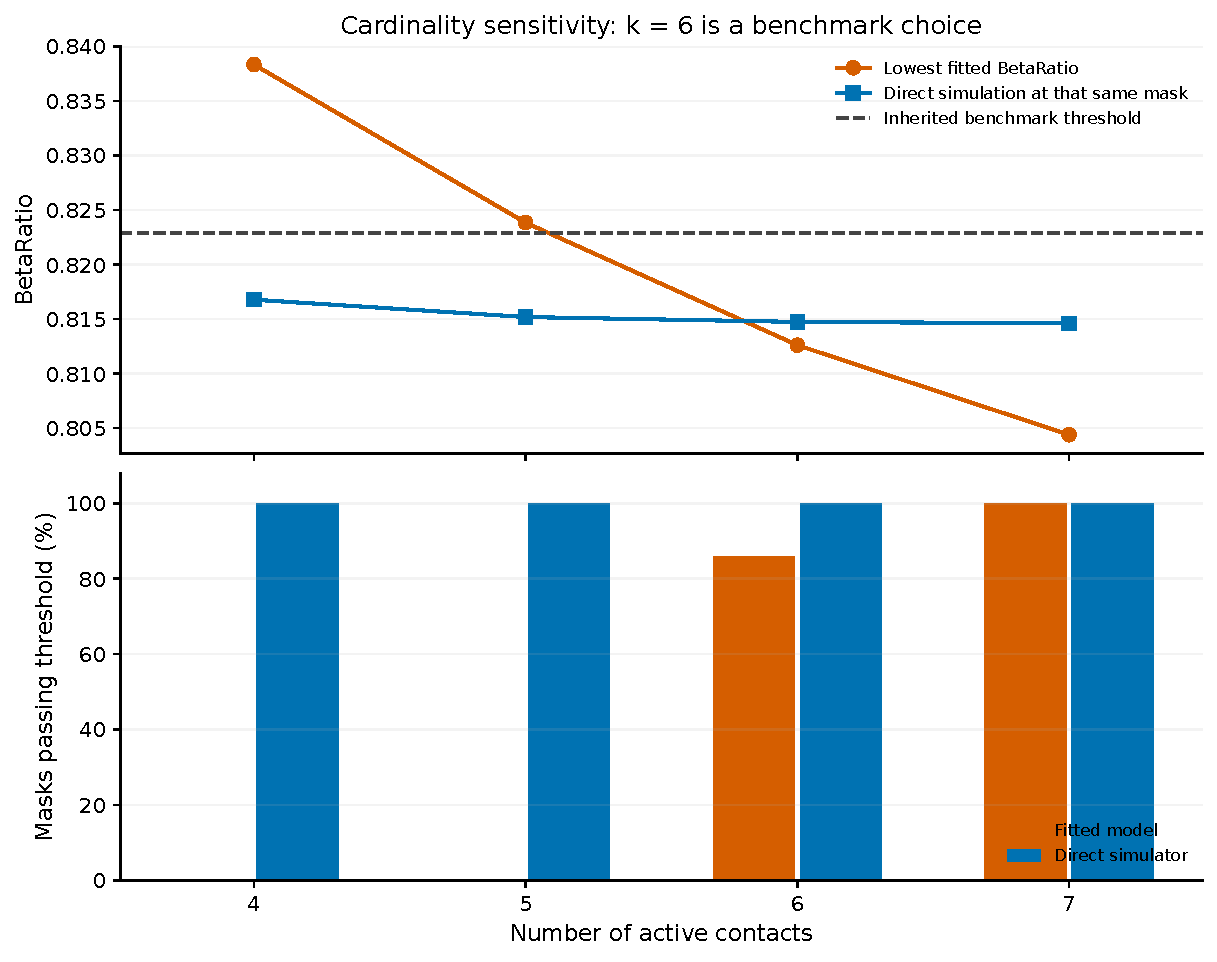
\includegraphics[width=0.9\textwidth]{figures/stage3_cardinality_sensitivity.pdf}
\caption{Cardinality sensitivity at $k=4,5,6,7$. Top: minimum fitted beta ratio at each cardinality and direct simulation at that same mask. Bottom: percentage of all $\binom{16}{k}$ masks passing each model's inherited efficacy threshold. The best fitted-beta mask need not minimize total objective. The figure tests model-dependent admissibility, not clinical contact necessity.}
\end{figure}
\begin{figure}[htbp]\centering
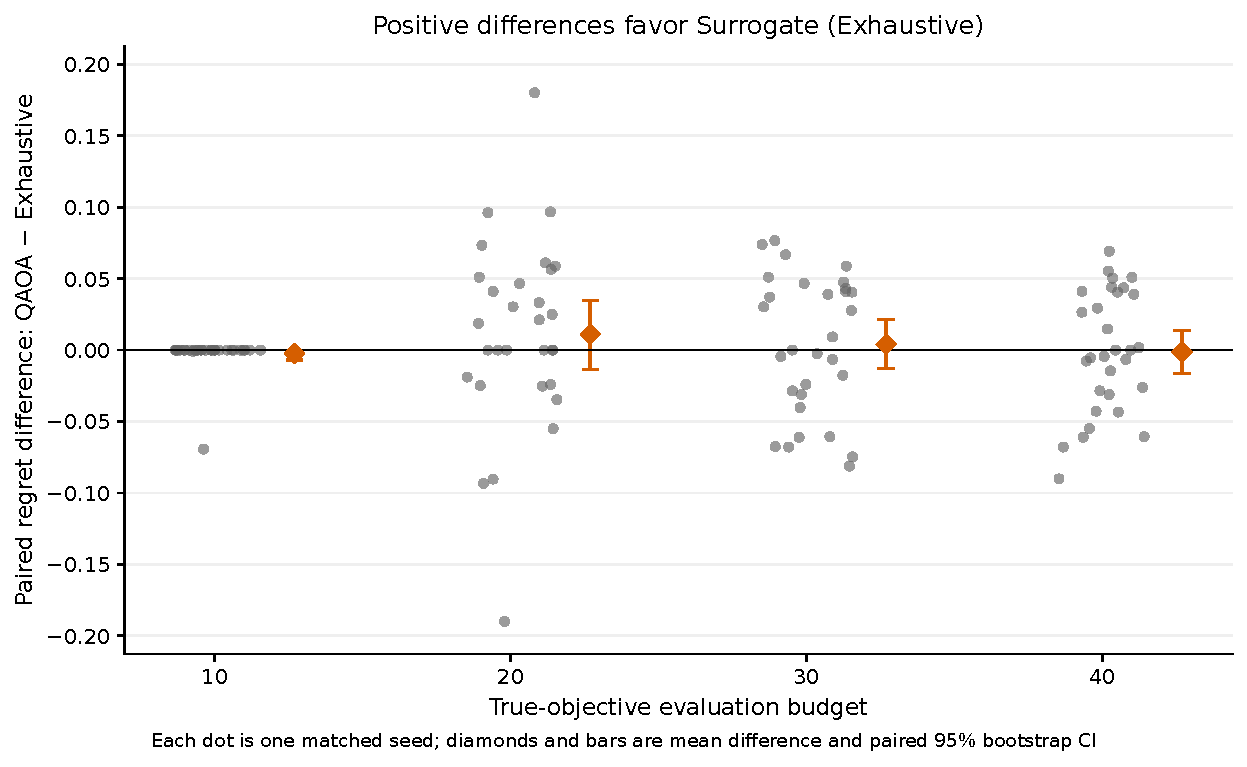
\includegraphics[width=0.9\textwidth]{figures/stage3_qaoa_vs_surrogate_exhaustive.pdf}
\caption{Per-seed paired regret differences, QAOA minus \fd. Negative favors QAOA. Diamonds are means with paired 95\% bootstrap intervals; the axis includes all observations and zero. Initial observations are identical but subsequent adaptive histories are independent. ``Exhaustive'' in the source artwork means full-domain surrogate prediction, not exhaustive objective evaluation.}
\end{figure}
\begin{figure}[htbp]\centering
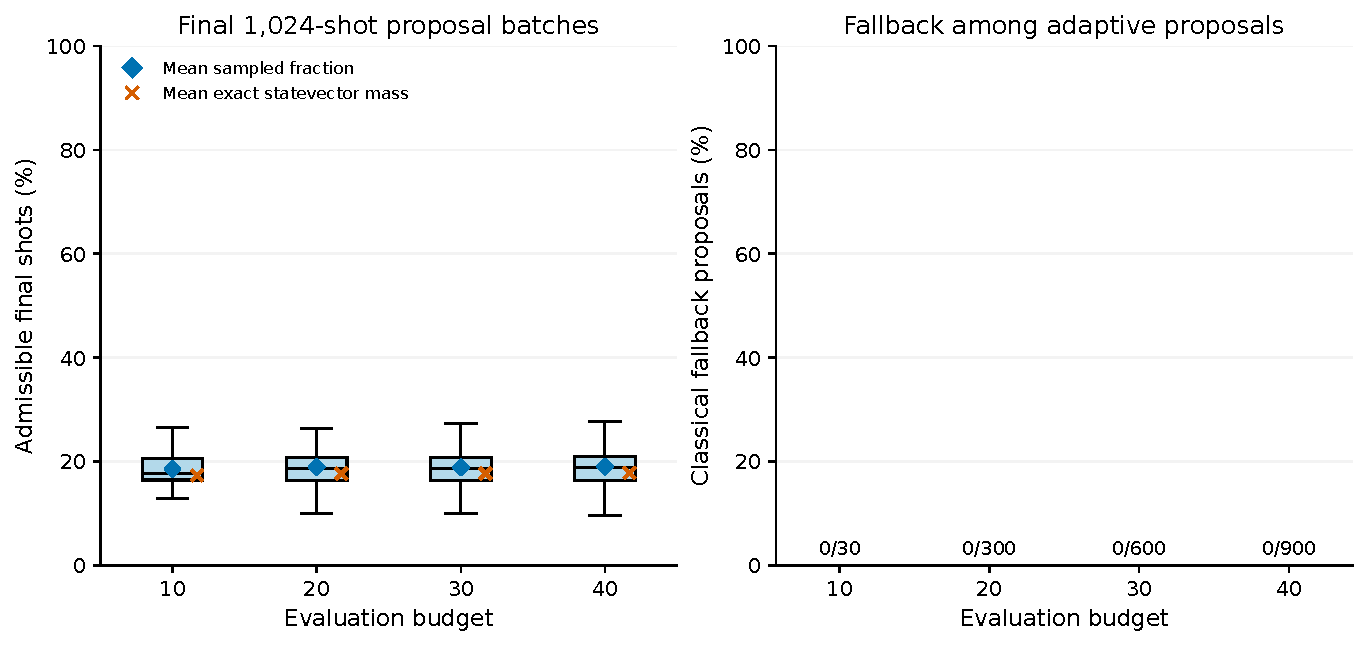
\includegraphics[width=0.93\textwidth]{figures/stage3_qaoa_feasibility_and_fallback.pdf}
\caption{QAOA final-batch admissibility and fallback. Left: distributions over final 1,024-shot batches (median, IQR, and 1.5-IQR whiskers; outlier markers omitted), mean sampled admissibility, and mean exact statevector admissible mass. Right: fallback counts/rates among adaptive proposals. Internal 256-shot angle-search batches are accounted for separately. Final selected objective queries are all admissible after filtering; this does not mean every raw sample is admissible.}
\end{figure}

\section{Frozen model and contact metadata}\label{app:params}
These parameters document the existing simulation and synthetic benchmark; they are not patient estimates. The decimal values below are drawn directly from the frozen notebooks. The repository is authoritative for numerical precision and execution details.
\begin{table}[htbp]\centering
\caption{Fixed deterministic STN--GPe simulation parameters from the frozen notebooks. Time constants and delays are in seconds.}\label{tab:params}
\small
\setlength{\tabcolsep}{4pt}
\begin{tabular}{lrrr}\toprule
Parameter & Value & Parameter & Value \\ \midrule
$\tau_s$ & 0.009480108684355502 & $\tau_g$ & 0.01568342986890998 \\
$d_{sg}$ & 0.005856049933455449 & $d_{gs}$ & 0.004355096988711622 \\
$w_{sg}$ & 0.8766085173129406 & $w_{gs}$ & 0.8007248587605185 \\
$I_c$ & 0.21584549577209655 & $I_g$ & 0.0 \\
$G_s$ & 2.418440027526686 & $G_g$ & 2.4195288944990088 \\
Initial $s,g$ & 0.1, 0.1 & Noise SD & 0.0 \\
\bottomrule\end{tabular}
\end{table}

\begin{table}[htbp]\centering
\caption{The single synthetic Stage 3 metadata instance. Contact indices imply no anatomical position. All factors are benchmark inputs.}\label{tab:metadata}
\small
\setlength{\tabcolsep}{4pt}
\begin{tabular}{lrrrr}\toprule
Index & Area factor & Impedance factor & Focus & Risk \\ \midrule
0 & 1.00 & 1.00 & 0.88 & 0.22 \\
1 & 1.00 & 1.02 & 0.92 & 0.20 \\
2 & 0.95 & 1.04 & 0.96 & 0.17 \\
3 & 0.95 & 1.06 & 1.00 & 0.14 \\
4 & 0.90 & 1.08 & 1.03 & 0.12 \\
5 & 0.90 & 1.10 & 1.01 & 0.13 \\
6 & 0.85 & 1.12 & 0.97 & 0.16 \\
7 & 0.85 & 1.14 & 0.93 & 0.19 \\
8 & 0.70 & 1.20 & 0.95 & 0.14 \\
9 & 0.68 & 1.24 & 1.02 & 0.11 \\
10 & 0.66 & 1.28 & 1.12 & 0.08 \\
11 & 0.64 & 1.32 & 1.22 & 0.06 \\
12 & 0.62 & 1.36 & 1.28 & 0.05 \\
13 & 0.60 & 1.40 & 1.18 & 0.07 \\
14 & 0.58 & 1.44 & 1.05 & 0.10 \\
15 & 0.56 & 1.48 & 0.96 & 0.13 \\
\bottomrule\end{tabular}
\end{table}

For the synthetic overlap matrix, let $d=\min(|i-j|,16-|i-j|)$. The base coefficient is 1.0, 0.45, or 0.15 when $d=1,2,3$, respectively, and zero otherwise. Multiply by 1.25 when both indices are in 0--7, by 0.70 when both are in 8--15, and by 1.0 for mixed groups. Historical ``ring'' and ``directional'' labels describe these synthetic groups only; they do not locate contacts in anatomy.
\begin{table}[htbp]\centering
\caption{Exact fitted-admissible optimum (mask 38180): preserved objective components. The omitted efficacy intercept is common to all masks and cancels from regret.}\label{tab:components}
\small
\setlength{\tabcolsep}{4pt}
\begin{tabular}{lr}\toprule
Component & Value \\ \midrule
Efficacy without $c_0$ & -0.12496052853010 \\
Count & 1.08000000000000 \\
Energy & 0.09325000000000 \\
Risk & 0.15400000000000 \\
Overlap & 0.36675000000000 \\
Charge-density soft term & 0.00000000000000 \\
Total & 1.56903947146990 \\
\bottomrule\end{tabular}
\end{table}

\end{document}
